\documentclass[11pt]{article}   % you have 10pt, 11pt, or 12pt options
\usepackage[margin=1in]{geometry}


\usepackage{physics}
\usepackage{amsmath}
\usepackage{amsmath,amsthm,amssymb,amsfonts,bbm,framed}
\usepackage{graphicx}
\usepackage{hyperref}
\usepackage{tikz}

\usetikzlibrary{bayesnet}
\usetikzlibrary{shapes,arrows}

\usepackage[url=false]{biblatex}
\bibliography{refs.bib}


%% custom macros
% vector
\newcommand{\V}[1]{\ensuremath{\boldsymbol{#1}}}
% matrix
\newcommand{\M}[1]{\ensuremath{#1}}
% math functions in non-italic font
\newcommand{\F}[1]{\ensuremath{\mathrm{#1}}}


\begin{document}  % necessary part of document


\title{Community Identification in Weighted Networks}
\author{Dan Kessler}

\maketitle

\begin{abstract}
  In this report we explore the problem of community identification in weighted networks under the stochastic block model (SBM).
  First, we introduce some important notation and ideas regarding graphs and networks and then providing background on the classical SBM.
  We then describe how it can be readily extended to the weighted case.
  The challenge and motivation for community identification is then introduced.
  We next provide a Bayesian formulation of the weighted SBM, and then review an approach using Variational Bayes (VB) to recover community identities and other parameters of interest.
  We then derive a Gibbs sampler as an alternative to the VB approach.
  Unfortunately, difficulties with the implementation precluded the inclusion of numerical results, but work on this project is ongoing as community detection in the weighted network setting will support current applied research projects involving brain imaging.
  We conclude by discussing limitations and speculate as to challenges inherent in the approach outlined in our sampler.
\end{abstract}

\section{Introduction}
\label{sec:introduction}

The investigation of the statistical properties of networks is a quickly growing field with many important applications.
While data analysis tasks in conventional statistical settings frequently require assumptions about independence, network data is fundamentally relational, as an observed network encodes relationships (edges) between units of observation (vertices).

While substantial prior work has focused on the statistical properties of binary networks, many modern applications involve networks that are most naturally considered weighted.
For example, in neuroscience, networks are frequently used to capture brain connectivity information, where edges represent some measure of dependence (frequently pairwise correlations of timeseries) between multiple locations in the brain, as captured with various brain imaging techniques (e.g., functional magnetic resonance imaging).

Many networks exhibit community structure, i.e., rather than treating each edge weight as following a unique distribution, one can group vertices in such a way that certain groups of edges become stochastically equivalent conditional on these groups.
A natural task, then, is to infer the community labels for a given network.

This report considers the problem of community detection in the weighted network setting for a particular class of generative networks models, i.e., the stochastic block model.

\section{Network Preliminaries and Notation}
\label{sec:netw-prel-notat}


Let $G=(V, E)$ be a graph, where $V$ is a set of vertices and $E \subseteq \left\{ (v, v') : v, v' \in V \right\}$ is a set of edges connecting some of the vertices in $V$.
In particular, if $(v, v') \in E$, then there is an edge linking vertex $v$ to vertex $v'$.
Suppose that $\lvert V \rvert = n < \infty$, i.e., we have $n$ vertices.
Without loss of generality, number the vertices $V$ as $1, 2, \ldots, n$.
In this case, we can represent the edge information using the adjacency matrix $A \in \left\{ 0, 1 \right\}^{n \times n}$, where $A_{i,j} = 1 \iff (i,j) \in E$.
See \autoref{fig:graphadj} for a graphical depiction of the relationship between graphs and their representation as adjacency matrices.

\begin{figure}[h]
  \centering
  \includegraphics[width=0.7\textwidth]{graphadj}
  \caption{Undirected Binary Graph and Adjacency Matrix from \href{https://cs.stackexchange.com/questions/71609/adjacency-matrix-and-recognizing-hierarchy}{Stack Exchange}}
  \label{fig:graphadj}
\end{figure}


While substantial prior work has focused on this problem in the classical setting where the network is a binary graph, i.e., edges are in $\left\{ 0,1 \right\}$, in this report we consider \emph{weighted graphs}, i.e., complete graphs where each edge has an attribute in $\mathbb{R}$.
We can naturally adjust the adjacency matrix such that now, $A \in \mathbb{R}^{n \times n}$, where the $i,j$ entry now captures the \emph{weight} of the edge linking the $i$'th and $j$'th vertices.






\section{Background: Stochastic Block Models}
\label{sec:backgr-stoch-block}
The stochastic block model (SBM) was first introduced by \textcite{holland_stochastic_1983} and is a frequently employed generative model used in the analysis of networks in a variety of settings.
Under the SBM, we suppose each $v \in V$ can be assigned to one of $K$ communities, i.e., let $\V{z} \in \left\{ 1, 2, \ldots, K \right\}^n$ give community assignments.
This assignment process is stochastic, with $z_i \overset{iid}{\sim} \operatorname{Categorical}(p_1, p_2, \ldots, p_K)$.
Conditional on $\V{z}$, the edges are independent with a distribution that depends only on the community memberships of the incident nodes, i.e., $\M{A}_{i,j} \mid \V{z} \overset{ind}{\sim} \operatorname{Bernoulli}(\M{P}_{z(i),z(j)})$, where
$\M{P} \in \left[ 0, 1 \right]^{K \times K}$ is a matrix of parameters that govern the probability of an edge for group of dyads.

It is possible to extend the SBM to the weighted case.
First, we suppose that all edges are present, i.e.,
$$E = \left\{ (i,j) : i \neq j, \in [n] \right\},$$ and as discussed above we let entries of $A$ take values in $\mathbb{R}$.
Rather than a Bernoulli likelihood for each edge's existence, we can consider a more general class of distributions, but for convenience we restrict ourselves to consideration of exponential families.
Now, we can replace the matrix of parameters $P$ with $\theta \in \mathbb{R}^{n \times n}$, and now $$\M{A}_{i,j} | \V{z} \overset{ind}{\sim} F(\M{\theta}_{z(i),z(j)}),$$ where $F$ is some law parameterized by $\M{\theta}$.




\section{Bayesian Formulation}
\label{sec:bayesian-formulation}

We follow a formulation laid out in \textcite{aicher_adapting_2013,aicher_learning_2015}.
As discussed above, we suppose that all edge distributions come from common exponential family, and we use conjugate priors for each of these parameters, i.e.,
\begin{equation*}
\pi_{\tau_r}(\theta_r) = \frac{1}{Z(\tau_r)} \exp(\tau_r \cdot  \eta(\theta_r)).
\end{equation*}
We then choose a flat prior for $\V{z}$:
\begin{equation*}
\pi_i(z_i) = \operatorname{Categorical}\left( \frac{1}{K}, \ldots, \frac{1}{K} \right).\label{eq:1}
\end{equation*}
Moreover, we assume $\V{z} \perp \V{\theta}$.
We can then write the prior as
$$\pi(z, \theta \mid \V{\tau}) = \prod_i^n \frac{1}{K} \prod_r^R \frac{1}{Z(\tau_r)} \exp( \tau_r \cdot \eta(\theta_r))$$.
Letting $\pi^{\star}(\V{z}, \M{\theta})$ be the posterior, we have
\begin{equation*}
  \pi^{\star} \propto P(A \mid \V{z}, \M{\theta}) \pi(\V{z}, \M{\theta}).
\end{equation*}


With this in place, the likelihood is given by
\begin{equation*}
  P(A \mid \V{z}, \theta) = \left[ \prod_{i < j}  h(A_{i,j}) \right] \exp( \sum_{i < j} T(A_{i,j}) \eta(\theta_{z_i,z_j}) ),
\end{equation*}
and the posterior by
\begin{equation*}
  \pi^{*}(\V{z},\M{\theta}) = \frac{P(\M{A} \mid \V{z},\M{\theta}) \pi(z) \pi(\theta)}{\int_{\Theta} \sum_{\V{z} \in \mathcal{Z}} P(\M{A} \mid \V{z}, \M{\theta}) \pi(\V{z}) \pi(\M{\theta}) d \theta}
\end{equation*}



\section{Variational Bayes Approach}
\label{sec:vari-bayes-appr}
Unfortunately, the posterior described above is presents substantial computational challenges due to the combinatorics invovled in integrating out over $\V{z}$.
\textcite*{aicher_adapting_2013,aicher_learning_2015} propose instead to approximate $\pi^{*}$ by a factorizable by a factorizable $q(\V{z},\M{\theta}) = q_{\V{z}}(\V{z}) q_{\M{\theta}}(\M{\theta})$, in particular
\begin{equation*}
  q(\V{z}, \theta \mid \V{\mu^{*}}, \V{\tau^{*}}) = \prod_i \mu_i^{*}(z_i) \times \prod_r \frac{1}{Z(\tau_r^{*})} \exp( \tau_r^{*} \cdot \eta(\theta_r)).
\end{equation*}
We wish to choose the $q$ with minimal KL-divergence with posterior:
\begin{equation*}
  \operatorname*{argmin}_q D_{KL}(q \parallel \pi^{\star}) = - \int q \log \frac{\pi^{\star}}{q}
\end{equation*}
While this minimization may seem especially difficult given the unpleasant nature of the posterior $\pi^{*}$, there's another way.
Recall that the marginal log likelihood of the data is a fixed quantity since $A$ has been observed.
Through manipulation, we obtain
  \begin{align*}
    C &= \log P(A) \\
    &= \int_{\Theta} \sum_{\V{z} \in \mathcal{Z}} q(\V{z},\theta) d\theta \log P(A) \tag{Multiply by 1}\\
              &= \int_{\Theta} \sum_{\V{z} \in \mathcal{Z}} q(\V{z},\theta) \log \frac{P(A, \V{z}, \M{\theta})}{P(\V{z}, \M{\theta} \mid A)} d\theta \tag{Conditioning tricks}\\
              &= \underbrace{\int_{\Theta} \sum_{\V{z} \in \mathcal{Z}} q(\V{z},\theta) \log \frac{P(A, \V{z}, \M{\theta})}{q(\V{z}, \theta)} d\theta}_{\mathcal{G}(q)}  \underbrace{- \int_{\Theta} \sum_{\V{z} \in \mathcal{Z}} q(\V{z}, \theta) \frac{P(\V{z}, \M{\theta} \mid A)}{q(\V{z}, \theta)} d\theta}_{D_{\text{KL}}(q \parallel \pi^{*})}
  \end{align*}
  Finally, we can rewrite the last result as
  \begin{equation*}
  D_{\text{KL}}(q \parallel \pi^{*}) = \underbrace{\log P(A)}_{\text{Constant}} - \mathcal{G}(q),
\end{equation*}
thus maximizing $\mathcal{G}$ minimizes the KL divergence as desired.

We can obtain some intuition for this approach by inspecting the form of $\mathcal{G}$:
\begin{align*}
  \mathcal{G}(q) &= \int_{\Theta} \sum_{\V{Z} \in \mathcal{Z}} q(\V{z}, \theta) \log \frac{P(A, \V{z}, \theta)}{q(\V{z},\theta)} d\theta \\
                 &= \int_{\Theta} \sum_{\V{Z} \in \mathcal{Z}} q(\V{z}, \theta) \log \frac{P(A \mid \V{z}, \theta) \pi(\V{z}, \theta)}{q(\V{z},\theta)} d\theta \\
                 &= \int_{\Theta} \sum_{\V{Z} \in \mathcal{Z}} q(\V{z}, \theta) \log P(A \mid \V{z}, \theta) d\theta + \int_{\Theta} \sum_{\V{Z} \in \mathcal{Z}} q(\V{z}, \theta) \log \frac{\pi(\V{z}, \theta)}{q(\V{z},\theta)}  d\theta \\
                 &= \mathbb{E}_q \left[ \log P(A \mid \V{z}, \theta) \right] + \underbrace{\mathbb{E}_q \left[ \log \frac{\pi(\V{z}, \theta)}{q(\V{z}, \theta)} \right]}_{-D_{\text{KL}}(q \parallel \pi)}.
\end{align*}
In the last line, we observe that we will be choosing a $q$ that maximizes our expected log likelihood, but that is regularized through the second term, which essentially penalizes deviation from the prior $\pi$.
\textcite{aicher_adapting_2013,aicher_learning_2015} note that as with many problems in Bayesian inference, given sufficiently large data, this first term will typically dominate and overwhelm the contribution of the prior.

\textcite{aicher_adapting_2013,aicher_learning_2015} present an iterative algorithm for maximizing $\mathcal{G}(q)$.
Briefly,  we have that 
\begin{align*}
G &\propto \sum_r^R  E_q (T_r + \tau_r - \tau_r^{*}) E_q(\eta(\theta_r)) + \sum_r^R \log \frac{Z(\tau_r)}{Z(\tau_r^{*})} + \sum_i + \sum_{z_i \in [K]} \mu_i^{*} \log \frac{\mu_i(z_i)}{\mu_i^{*}(z_i)} \\
  E_q T_r &= \sum_{i < j} \sum_{(z_i, z_j) = r} \mu_i^{*}(z_i) \mu_j^{*} (z_j) T(A_{i,j}) \\
  E_q \eta(\theta_r) &= \frac{\partial }{\partial {\tau}} \log Z({\tau}) \left. \right|_{\tau = \tau_r^{*}},
\end{align*}
and by taking gradients we can obtain update rules.
MATLAB code for this algorithm is provided by the authors \href{http://tuvalu.santafe.edu/~aaronc/wsbm/}{online}.


\section{Sampling-Based Approach}
\label{sec:sampl-based-appr}

We wished to explore a sampling-based approach in addition to the VB approach outlined above.
\Textcite{snijders_estimation_1997} propose a Gibbs sampler for the setting of the undirected SBM with binary edges, which we extend to the weighted case.
Their notation differs from (and directly conflicts with) the conventions in \parencite{aicher_adapting_2013,aicher_learning_2015}, so our treatment here modifies their notation to be internally consistent.

First, we use a slightly extended form of the model introduced in \autoref{sec:bayesian-formulation}, where we will put a prior on $\mu$.
Since the likelihood of $\V{z} \mid \mu$ is multinomial\footnote{or with some notational adjustment, categorical}, choosing a Dirichlet prior with hyperparameter $\alpha$ is a natural choice that gives conjugacy.
Like the model from \textcite{aicher_adapting_2013,aicher_learning_2015}, our approach can be readily generalized to exponential family likelihoods for $A$ in general, for notational compactness we consider the case where the likelihood of $A$ is normal with known (unit) variance, i.e., $A_{i,j} \mid \theta, \V{z} \sim N(\theta_{z_i,z_j},1)$, in which case it is natural to choose a normal distribution as the prior for $\theta$ with hyperparameters $\mu_0$ and $\sigma^2_0$ in order to achieve conjugacy, i.e., $\theta_{i,j} \sim N(\mu_0, \sigma_0^2)$.
A graphical depiction of our model is presented in \autoref{fig:plate-overview}.


Adapting their approach, we arrive at two-step sampler.
Assuming we index our samples by $p$, and supposing we have current values  $\mu^{(p)}, \theta^{(p)}, \V{z}^{(p)}$, we first draw $(\theta^{(p+1)}, \mu^{(p+1)}$ from the conditional distribution $(\theta, \mu \mid Z^{(p)}, A)$.
Next, we iterate through the components of $\V{z}$, and draw each conditional on all the other $\V{z}$ (using any new draws in the present step where possible),

In particular, our approach involves the following.
% First, $\theta \mid \V{Z}, A, \mu \overset{d}{=} \theta \mid \V{Z}, A$, by d-separation argument from the DAG, see \autoref{fig:plate-overview}).
yLetting $n_{i,j}$ denote the number of edges in the $i,j$ block and letting $t_{i,j}$ denote the sum of the edges in the $i,j$ block (with blocks defined based on the current $Z$), by conju
% by conjugacy $\theta_{i,j} \mid \V{Z}, A; \mu_0, \sigma_0^2 \sim N( \left( \frac{1}{\sigma_0^2 + \frac{n_{i,j}}{\sigma^2} \right)^{-1} \left( \frac{\mu_0}{\sigma_0^2} + \frac{t_{i,j}}{\sigma^2} \right)$, so this update is straightforward.

Next, 


R code implementing this procedure is available on \href{https://github.com/dankessler/608b-project}{github}, along with a short script that conducts a proof-of-concept numerical experiment.\footnote{Whilte the code presently ``works'', i.e., produces results and not errors, the author believes that the current implementation is incorrect, as the results obtained are fairly nonsensical. The code will be updated as the author continues to work to implement this sampler so that it can be integrated into their broader research.}


\begin{figure}[h]
  \centering
  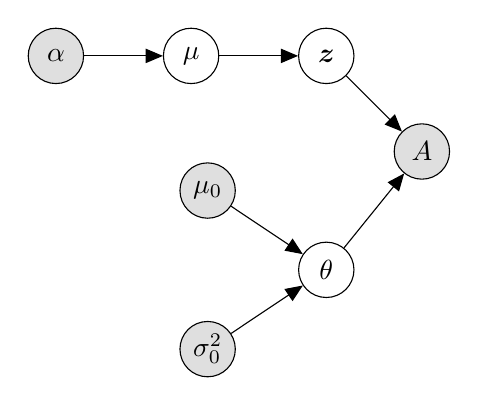
\begin{tikzpicture}
    
    % using BayesNet library: https://github.com/jluttine/tikz-bayesnet

    % Nodes first I guess

    \node[obs] (a) {$\alpha$};
    \node[latent, right=of a] (u) {$\mu$};
    \node[latent, right=of u] (z) {$\V{z}$};
    \node[obs, below right=1 of z] (A) {$A$};
    \node[latent, below=2 of z] (t) {$\theta$};
    \node[obs, above left=0.5 and 1 of t] (u0) {$\mu_0$};
    \node[obs, below left=0.5 and 1 of t] (s0) {$\sigma_0^2$};

    % Set up plate
    % \plate {subs} {(y) (B) (th) (A) (X)} {N};

    % dot products


    % wire up edges
    \edge[->]{z,t}{A};
    \edge[->]{a}{u};
    \edge[->]{u}{z};
    \edge[->]{u0}{t};
    \edge[->]{s0}{t};
    % \edge[->]{W, B, beta, th, sig2}{y};
    % \edge[->]{B,c}{A};
    % \edge[->]{th,c}{X};



  \end{tikzpicture}  
  \caption{Graphical depiction of generative model. Grayed nodes are observed (or fixed hyperparameters), white nodes are latent.}
  \label{fig:plate-overview}
\end{figure}

\section{Discussion}
\label{sec:discussion}



The data that I consider in my research  is motivated by applications in cognitive neuroscience and is related to the networks generated by the stochastic block model, but with several important extensions.
First, I have been studying cases where we observe a \emph{sample} of networks on a common node set (or where the node set can be meaningfully registered across observations.
Second, the networks that I study are typically (i) dense, (ii) weighted, and (iii) signed.
Finally, I consider cases where in addition to observing the adjacency matrices $A^{(i)}$, we also observe nodal attributes $X^{(i)} \in \mathbb{R}^{n \times p}$, where $p$ is the number of covariates observed at each node.

While my current projects are largely focused on predicting observation-specific labels ($y_i)$ using $(A_i,X_i)$, in that work we currently consider $c$ fixed, known, and shared across all observations.
However, in future iterations of the project I intend to consider cases where $c$ is considered unknown or possibly cases where $c$ varies across the sample.




\printbibliography

\end{document}



%%% Local Variables:
%%% mode: latex
%%% TeX-master: t
%%% End:

% LocalWords:  variational
